\documentclass[a4paper]{article}

\usepackage[english]{babel}
\usepackage[utf8]{inputenc}
\usepackage{amsfonts}
\usepackage{amssymb}
\usepackage{amsmath}
\usepackage{graphicx}
\usepackage[colorinlistoftodos]{todonotes}
\usepackage{titling}
\usepackage{listings}
\usepackage[T1]{fontenc}
\usepackage{array,multirow,makecell}
\setcellgapes{1pt}
\makegapedcells
\newcolumntype{R}[1]{>{\raggedleft\arraybackslash }b{#1}}
\newcolumntype{L}[1]{>{\raggedright\arraybackslash }b{#1}}
\newcolumntype{C}[1]{>{\centering\arraybackslash }b{#1}}

\newcommand{\subtitle}[1]{%
  \posttitle{%
    \par\end{center}
    \begin{center}\large#1\end{center}
    \vskip0.5em}%
}
\lstset{%
  basicstyle=\scriptsize\sffamily,%
  commentstyle=\footnotesize\ttfamily,%
  frameround=trBL,
  frame=single,
  breaklines=true,
  showstringspaces=false,
  numbers=left,
  numberstyle=\tiny,
  numbersep=10pt,
  keywordstyle=\bf
}





%%%%%%%%%%%%%%%%%%%%%%%%%%%%%%%%%%%%%%%%%%%%%%%%%%%%
% Raport Headers:
%%%%%%%%%%%%%%%%%%%%%%%%%%%%%%%%%%%%%%%%%%%%%%%%%%%%
\title{Image and signal processing: Computer exercise 4\\CE04G02T05}
\author{PASHEVICH Alexander, SID-LAKHDAR Riyane}
\date{15/11/2015}

\begin{document}
% Beginning serious stuff.


\maketitle
% Actually prints title / subtitle / authors and dat into the document


%%%%%%%%%%%%%%%%%%%%%%%%%%%%%%%%%%%%%%%%%%%%%%%%%%%%
% Abstract
%%%%%%%%%%%%%%%%%%%%%%%%%%%%%%%%%%%%%%%%%%%%%%%%%%%%
\begin{abstract}
This report summarize, explains and refers to the answers we have designed for the fourth ''Image and Signal Processing'' computer exercise. This paper refers to exploring of spatial frequency scale and spatial structures as well as filters in the Fourier domain. During the work we made experiments, tested the theory and explored the result which is represented below.
\end{abstract}

%%%%%%%%%%%%%%%%%%%%%%%%%%%%%%%%%%%%%%%%%%%%%%%%%%%%
% Introduction
%%%%%%%%%%%%%%%%%%%%%%%%%%%%%%%%%%%%%%%%%%%%%%%%%%%%
\section{Introduction}
The aim of this report is to describe the relation between the spatial frequency scale of a signal and its spatial structure. This link will be studied thanks to one of the most important tool in signal processing: the Fourier transform. This function is an obvious choice to solve such a problem as it transforms a spacial domain function into a frequency domain function.   In this report, we will only consider 2 dimensional discrete functions.\\\\
Once we will have considered ways to study the frequency(s) of a signal, we will study a mathematical tool called filters used to transform a signal (sum of signals with different frequencies) into the same signal where some specific constituent signals have been removed (regarding to them frequencies).



\section{Material \& Methods}
    \subsection{Spatial Frequency Scale and Spatial Structures}
        \subsubsection{Two dimensional Fourier transform: frequency function}
        The two dimensional Fourier transform of a discrete two dimensional function f is defined as: $\sum_{x=0}^{w}{\sum_{y=0}^{h}{f(x, y)e^{-i 2 \pi(u x + v y)}}}$.\\
        This transform maps a function defined on a spatial domain to a function defined on a frequency domain.   In this report, we will try to deduce frequency properties
        on the 2 dimensional Fourier transform.   Then we will try to link this properties with spatial properties on the initial function.



        \subsubsection{Spatial property}
        Let S the sum of all the pixels of an image, and let $(u_{0}, v_{0})$ the couple of frequencies such as $F(u_{0}, v_{0}) = S$
        \begin{equation*}
        \begin{aligned}
          F(u_{0}, v_{0}) &= \sum_{x=0}^{w}{\sum_{y=0}^{h}{f(x, y)}} \\
          \sum_{x=0}^{w}{\sum_{y=0}^{h}{f(x, y)e^{-i 2 \pi(u_{0} x + v_{0} y)}}}&= \sum_{x=0}^{w}{\sum_{y=0}^{h}{f(x, y)}}
        \end{aligned}
        \end{equation*}
        As the function f and the exponential function are both positive, this equation means that $e^{-i 2 \pi(u_{0} x + v_{0} y)} = 1 \text { } \forall (x, y) \in \mathbb{R} ^{2}$. Thus, the 2 frequency indexes (u,v) where the Fourier Transform of an image equals the sum of all the pixels in the spatial domain are (0, 0).\\\\
        As we are dealing with finite discrete signal, we can experimentally check this previous property by running the loop Figure Fig \ref{solve_discret_equation.py} on the all the possible input of a Fourier transform and checking if the output of the function corresponds to the expected sum.
        \begin{figure}[ht!]
	    \lstset{language=Python}
	    \begin{lstlisting}
# return the list of solutions (u, v) such as ft2D(u, v) = s
def solve_discret_equation(ft2d, s):
    res = []
    for x in xrange(len(ft2d)):
        for y in xrange(len(ft2d[0])):
            if ft2d[x, y] == s:
                res.append((x, y))
    return res
        \end{lstlisting}
        \caption{Python code to solve an equation on a 2D function.}
	    \label{solve_discret_equation.py}
		\end{figure}



        \subsubsection{Frequency property}
        The Fourier transform of an image may be interpreted using several complex number representation.  The one we will mainly use in this report is the exponential one: (magnitude, phase).\\
        Let consider the spectrum operator.   This mathematical operator computes the logarithm of the squared modulus (magnitude) of complex function.   The program in the figure \ref{spectrum2D.py} computes the spectrum of a given 2D complex input function (2D Fourier transform).

        \begin{figure}[h!]
	    \lstset{language=Python}
	    \begin{lstlisting}
def power_spectrum_2D(ft2d, fx=None, fy=None):
    epsilon = np.finfo(float).eps
    if fx != None:
        res = np.zeros(len(ft2d[0]))
        for y in xrange(len(ft2d[0])):
            val             = ft2d[fx, y]
            magnitudeSquare = val.imag * val.imag + val.real * val.real
            res[y]          = np.log(magnitudeSquare + epsilon)
        return res

    if fy != None:
        res = np.zeros(len(ft2d))
        for x in xrange(len(ft2d)):
            val             = ft2d[x, fy]
            magnitudeSquare = val.imag * val.imag + val.real * val.real
            res[x]          = np.log(magnitudeSquare + epsilon)
        return res

    res = np.zeros(ft2d.shape)
    for x in xrange(len(ft2d)):
        for y in xrange(len(ft2d[0])):
            val             = ft2d[x, y]
            magnitudeSquare = val.imag * val.imag + val.real * val.real
            res[x, y] = np.log(magnitudeSquare + epsilon)
    return res
        \end{lstlisting}
        \caption{Python code to compute the spectrum of a 2D function.}
	    \label{spectrum2D.py}
		\end{figure}
        In the ''Experiments'' section, we will see how this algorithm, applied to different images (with different spatial properties) allows us to determine the frequency properties of this pictures and to decompose an image into signals depending on them frequencies.

	\subsection{Filters in the frequential domain}
    	\subsubsection{Filters' descriptions}
The filters used in the computer exercise are defined below.\\
The first filter is called cylinder and it is defined with the formula \ref{cylinder}. It has one parameter which is called cut off frequency ($f_c$).
\begin{equation}
\label{cylinder}
H_F(f_x,f_y) = \begin{cases}
               1 & \text{if } \sqrt{f_x^+f_y^2} < f_c\\
               0 & \text{otherwise}
            \end{cases}
\end{equation}
The Butterworth filter is defined with formula \ref{butterworth}. In addition to the cut off frequency it also has a parameter of order ($n$).
\begin{equation}
\label{butterworth}
H_F(f_x,f_y)=\frac{1}{1 + (\frac{\sqrt{_x^2+f_y^2}}{fc})^{2n}}
\end{equation}
The last filter is called gaussian and it is one of the most known and widely used filters. It has two parameters: sigmas for x and for y which are standard deviations for both axes.
\begin{equation}
H_F(f_x,f_y)=e^{-\frac{f_x^2}{2\sigma_x^2}-\frac{f_y^2}{2\sigma_y^2}}
\end{equation}
The code which implements those filters is given in figure \ref{filters_code}. To apply those filters to original image $I$ we use the formula:
\begin{equation}
\label{filter_formula}
I_{filtered} = F^{-1}(H) \text{ where } H(f_x, f_y) = H_F(f_x, f_y) * F(I)(f_x, f_y)
\end{equation}
If we would like to introduce the notion of cut off frequency while working with gaussian filter, we would like the following formula to be true $H_F(f_c,0)=H_F(0,f_c)=\frac{1}{2}$. From the formula we can deduce the value of $\sigma_x=\sigma_y$.
\begin{equation*}
H_f(f_c,0)=e^{-\frac{f_c^2}{2\sigma_x^2}}=\frac{1}{2}=e^{ln\frac{1}{2}} \Rightarrow \sigma_x = \frac{f_c}{\sqrt{2ln2}}
\end{equation*}
Exactly the same applies to $\sigma_y$ so in this case $\sigma_x = \sigma_y$.
		\subsubsection{Implementation}
\begin{figure}[ht!]
\lstset{language=Python}
\begin{lstlisting}
def cylinder_filter(Nx, Ny, cutOffFrequency, typeFilter):
    res = np.zeros((Nx, Ny))
    for x in range(Nx):
        for y in range(Ny):
            fx = 1. * x / Nx
            fy = 1. * y / Ny
            if np.sqrt(fx ** 2 + fy ** 2) <= cutOffFrequency:
                res[x, y] = 1
            else:
                res[x, y] = 0
    return res


def butterworth_filter(Nx, Ny, cutOffFrequency, n):
    res = np.zeros((Nx, Ny))
    for x in range(Nx):
        for y in range(Ny):
            fx = 1. * x / Nx
            fy = 1. * y / Ny
            res[x, y] = 1. / (1 + (np.sqrt(fx ** 2 + fy ** 2) / cutOffFrequency) ** (2 * n))
    return res


def gaussian_filter(Nx, Ny, sigma_x, sigma_y):
    res = np.zeros((Nx, Ny))
    for x in range(Nx):
        for y in range(Ny):
            fx = 1. * x / Nx
            fy = 1. * y / Ny
            res[x, y] = np.exp(- 0.5 * (fx ** 2) / (sigma_x ** 2) - 0.5 * (fy ** 2) / (sigma_y ** 2))
    return res
\end{lstlisting}
\caption{Python code for filters' implementation}
\label{filters_code}
\end{figure}

















\section{Experiments}
	\subsection{Experimental setup}
	In this report, we only use the provided pictures.   This images and some of them graphical properties will be given in this section.   We will also use our previously defined algorithm to find some of the frequency properties.
    \subsection{Spatial Frequency Scale and Spatial Structures}
    
    	\subsubsection{Fourier transform: symmetry on image}
        For images, generally, the 2D Fourier Transform is centered around zero.   This symmetry property is clearly shown on the figure Fig \ref{wheeleSpectrum.pgm} (right picture).\\
         In fact this symmetry is not according to the central coordinate of the picture (transcribed to frequencies) but is according to a period of size (w, h) where w is the width of the picture and h its height.   However, this picture clearly shows that a period starts at (0, 0).   Thus, in the following spectrum we will describe, we will consider power spectrum in the usual form (the null frequency at the center of the Fourier matrix).\\




		\subsubsection{Spectrum interpretation}
        First of all, we applied the spectrum program given in the "Material \& methods" section to the picture in the figure \ref{wheeleAndSpectrum.pgm} (left picture).   The result is represented in the same figure (right picture).
         \begin{figure}[!htb]\centering
             \begin{minipage}{0.45\textwidth} \frame{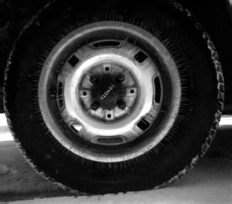
\includegraphics[width=\linewidth]{wheele.png}} \end{minipage}
             \begin{minipage}{0.45\textwidth} \frame{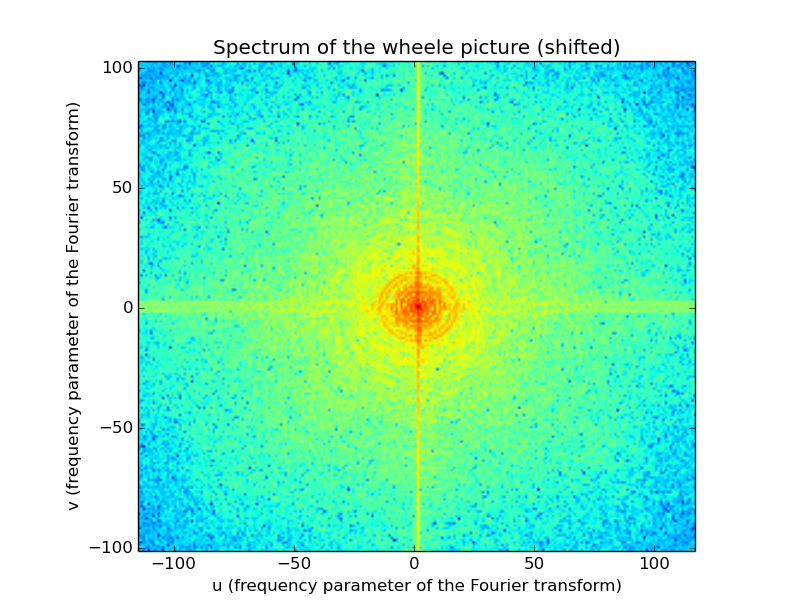
\includegraphics[width=\linewidth]{wheeleSpectrumShifted.png}} \end{minipage}
             \caption{Black and white picture and its corresponding spectrum}
             \label{wheeleAndSpectrum.pgm}
         \end{figure}

        An image is the sum of signals $s_{\phi}$ where $\phi$ is the frequency of the signal.\\
        We can observe on this spectrum that the small frequencies (u or v close to zero) have a very important magnitude compared to the others.  This means that small frequency signals that compose the initial image are much more significant that the high frequency signals.   What we mean here by "significant" is that mainly the original image consists of those low frequencies (of the 2D signals which correspond to them) and if we remove the high frequencies we will not loose a lot of information. So removing the low frequencies signals from the image means lost of a lot of details while removing other signals (with a higher frequency) would have less impact on the quality of the image.\\\\
After we retrieved the Fourier coefficients and calculated the magnitude, we applied the inverse Fourier transform and received the same image which is not surprising actually as according to the theory $I = F^{-1}(F(I))$.\\\\
        Let's now consider the picture and its spectrum in the figure \ref{chessBoardAndSpectrum.pgm}. This picture has some obvious spatial periodicity properties. But how does this properties affect the frequency properties of the picture?

         \begin{figure}[!htb]\centering
             \begin{minipage}{0.45\textwidth} \frame{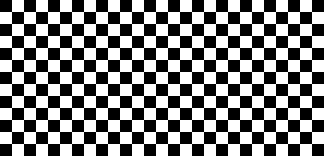
\includegraphics[width=\linewidth]{damierHV.png}} \end{minipage}
             \begin{minipage}{0.45\textwidth} \frame{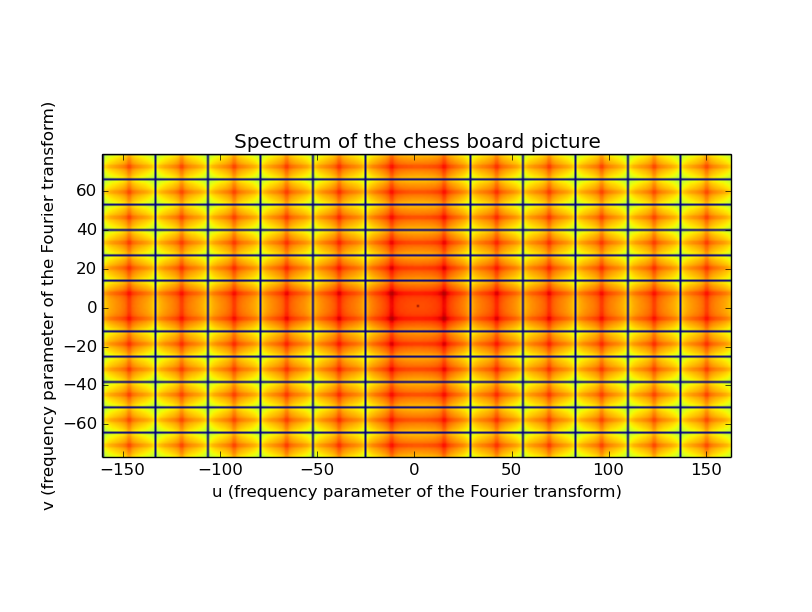
\includegraphics[width=\linewidth]{chessBoardSpectrum.png}} \end{minipage}
             \caption{Black and white picture and its corresponding spectrum}
             \label{chessBoardAndSpectrum.pgm}
         \end{figure}

         First of all, we can notice that the spectrum alternates high and low magnitudes over $f_{x}$ (horizontal frequency axes) and $f_{y}$ (vertical frequency axes) with the same fixed period.  This allows us to determine frequency coordinates for the first frequency peak at ($f_{x} = 15, f_{y} = 6$).\\\\
         Secondly, we can notice that the red color is highly dominant (frequencies with high magnitude).   Thus the contrast between colors is extremely high in most of the picture.
         We also notice extremely low magnitude (periodically) which correspond to spaces where the picture has the same color with no contrast.   
         Finally, we can notice that the alternation between high and low magnitudes (over horizontal or vertical axes) are not strict (there are shadings between red and blue magnitudes).   
         Thus, the break lines between white and black colors in the original picture are not strict and contain gray pixels.


		\subsubsection{Fixing a frequency in the spectrum: 1D frequency function}
        For a given fixed frequency ($f_{x}$ or $f_{y}$), we want now to determine the behavior of the Fourier transform depending on the other frequency.   Using the program described in the "Materials \& Methods" section, we have represented on the figure \ref{fixedFrequency.pgm} the spectrum power when we have fixed the $f_{x}$ frequency (left figure) and the $f_{y}$ frequency (right figure).\\\\
         \begin{figure}[h!]\centering
             \begin{minipage}{0.45\textwidth} \frame{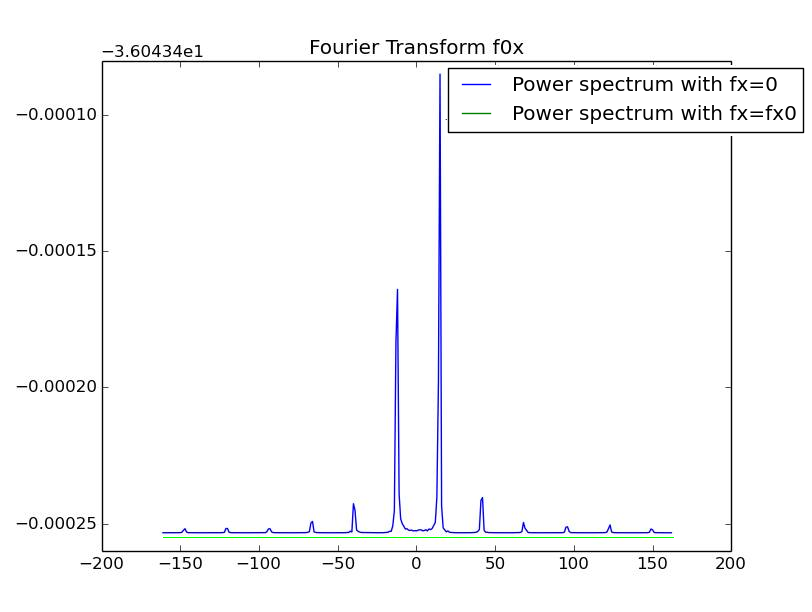
\includegraphics[width=\linewidth]{powerSpectrum_fxFixed.png}} \end{minipage}
             \begin{minipage}{0.45\textwidth} \frame{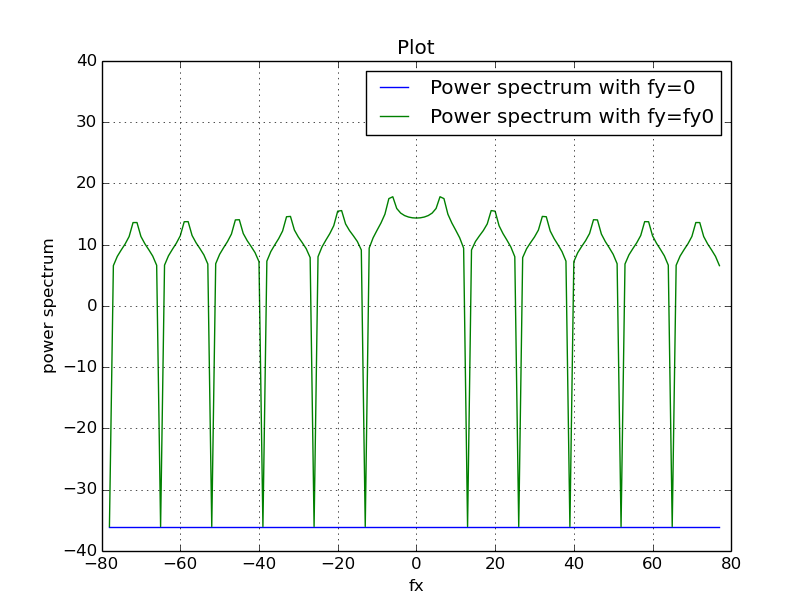
\includegraphics[width=\linewidth]{powerSpectrum_fyFixed.png}} \end{minipage}
             \caption{1D spectrum with a fixed second parameter (chess board image)}
             \label{fixedFrequency.pgm}
         \end{figure}
        This figures confirm the results of the 2D spectrum (figure \ref{chessBoardAndSpectrum.pgm}): For the line ($f_{y} = 0$) of the spectrum, the peak and the holes of the spectrum are perfectly matching the peak and the holes of the 1D function for $f_{y} = 0$ fixed.  This checking may successfully be done for all the other value of fixed $f_{x}$ and $f_{y}$.\\

		\subsection{Filters in the frequential domain}
When we apply filters to an image, we changes Fourier coefficients using the formula \ref{filter_formula}. Normally, we remove either high frequencies (\textit{Low pass filters}) or low frequencies (\textit{High pass filters}) by removing (setting them to null) Fourier coefficients with high or low indexes correspondingly. Some filters don't completely remove those coefficients but instead of it they multiply the coefficients by very small number. If we remove high indexes, we see only low frequencies which means that the image looses clearness and becomes blurred. However we can still see the main contours. In case of high pass filters, we do exactly the opposite. We loose most of the sensible information however acquire some additional information about rapid drops of color for example. Anyway in both cases we loose some information on the image in order to concentrate on different aspects of it.\\\\
We can see the results of applying of the cylinder filter which is given by formula \ref{cylinder} on the classical image of Lena on the figure \ref{filtered_images}. We used the filter with cut off frequency $f_c = \frac{1}{16}$. As we can see, the image became blurred however we still can understand what is shown on it. We also show the image filtered by gaussian and butterworth filters and also the original one. As we can see, the gaussian and butterworth filters do pretty much the same that the cylinder. They blur the image by reducing high frequencies. However, they do not completely remove them. Instead of this they reduce values of Fourier coefficients for high frequencies which actually do pretty much the same.
\begin{figure}
    \centering
    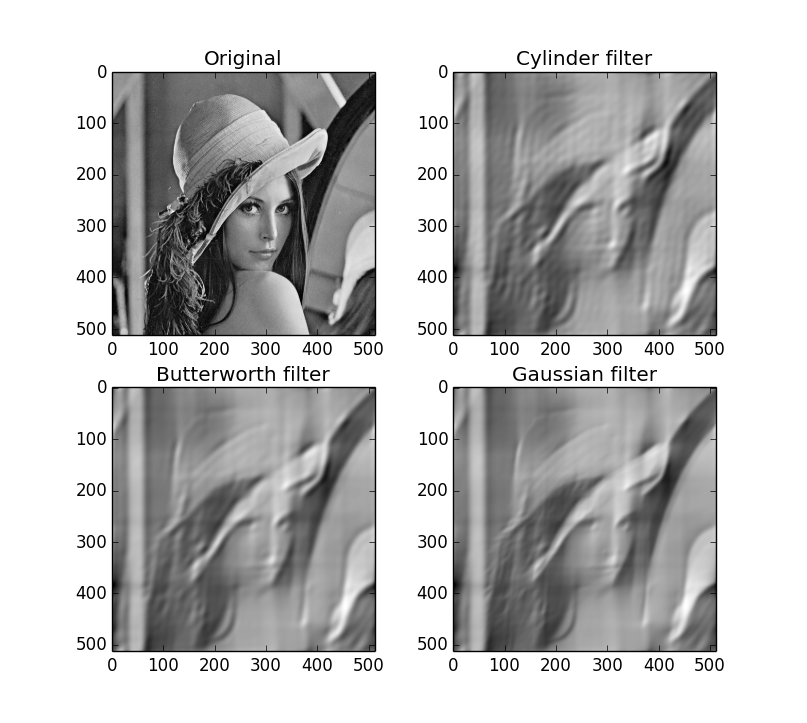
\includegraphics[width=0.7\textwidth]{filtered_images.png}
    \caption{Original and filtered images}
    \label{filtered_images}
\end{figure}
Filters are represented in the figure \ref{filters}. Those images are plots for $H_F$ with fixed $f_y=0$. From the image it is clear that the cylinder filter just removes every frequency which is higher than some $f_{max}^x$. If we look at the formula \ref{cylinder}, we can deduce that $f_{max}^x = f_c * N_x = \frac{512}{16} = 32$ for our case. The rest of frequencies stay without changes. In case of butterworth and gaussian filters the filter becomes smooth (it means that we can take derivative of it which is big advantage). However, as we can deduce from the figure the butterworth filter does almost the same with the cylinder. Frequencies higher than 30-40 are almost neglected (which also corresponds to $f_c * N_x$). Gaussian filter takes into account frequencies lower than 90.\\\\
\begin{figure}
    \centering
    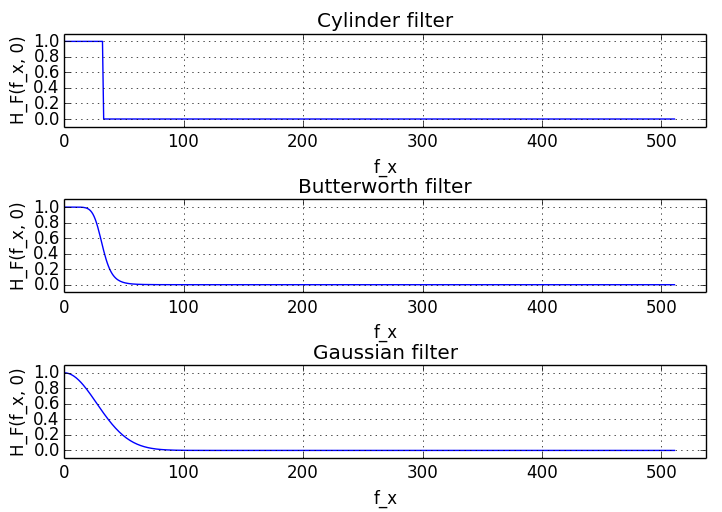
\includegraphics[width=0.7\textwidth]{filters.png}
    \caption{Filters}
    \label{filters}
\end{figure}
1D impulse responses are represented in the figure \ref{impulse_responses}. The pictures are the same but on the second only first 50 samples are shown for the sake of zooming in. As it can be seen, in the original image most of frequencies are negligibly small. However, the highest frequencies are quite dense and the filters completely diminish them which makes the filtered image low blurred. We also can deduce from the image that the filters do pretty much the same job without looking at the outputs.
\begin{figure}[!htb]\centering
\begin{minipage}{0.49\textwidth} \frame{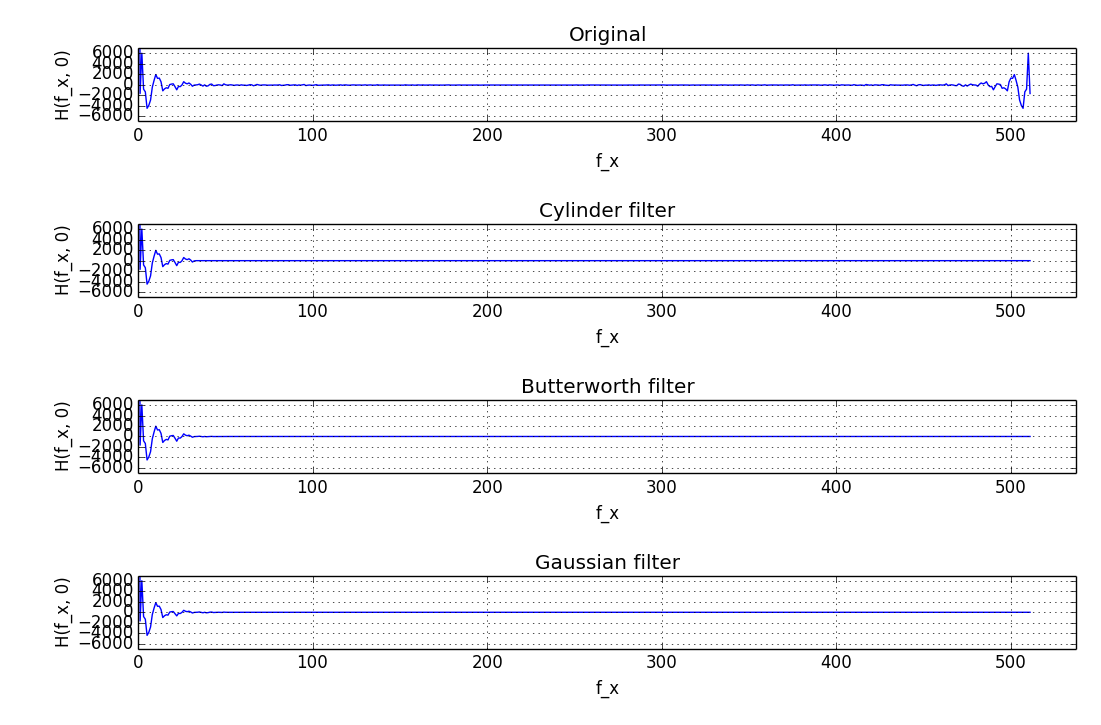
\includegraphics[width=\linewidth]{filtered_ft_1.png}} \end{minipage}
\begin{minipage}{0.49\textwidth} \frame{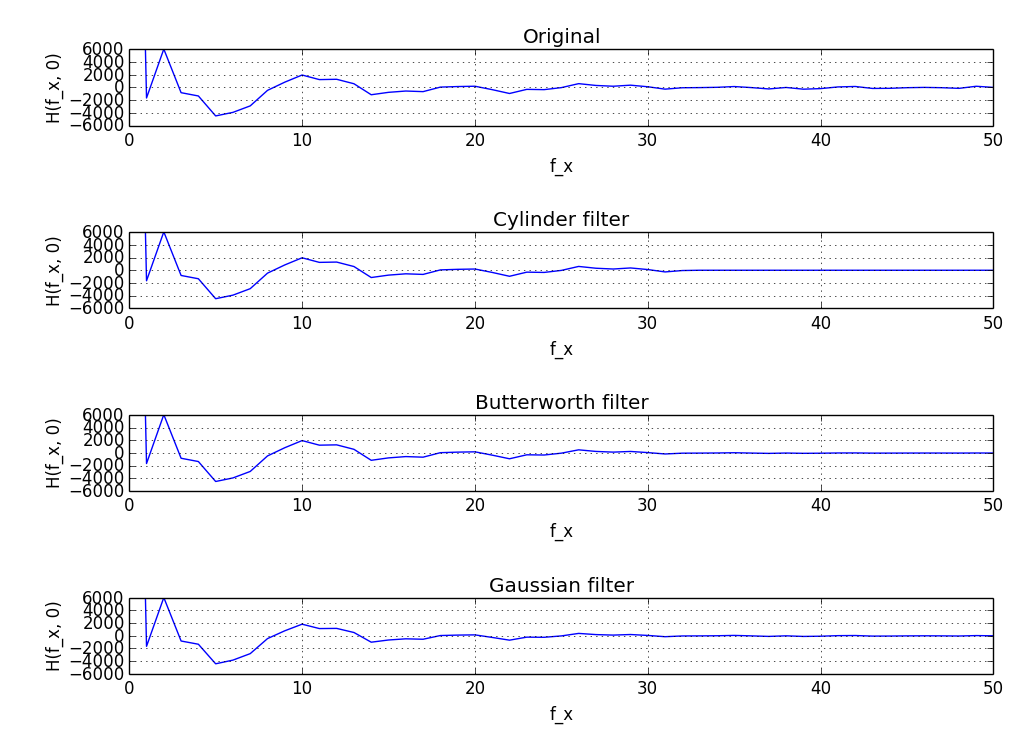
\includegraphics[width=\linewidth]{filtered_ft_2.png}} \end{minipage}
\caption{1D impulse responses for the filters}
\label{impulse_responses}
\end{figure}




\section{Conclusion}
During the work on the lab exercises, we worked with Fourier transform and explored spatial properties of some images. We also used filters to change the spatial properties of input images. We implemented the used methods using Python programming language as well as understood how Fourier transform of 2D signals work and what different frequencies and their magnitude means. To conclude, this lab exercises gave us insight how Fourier transform of 2D signals works and what their spatial properties mean.




\end{document}
